\documentclass[11pt]{article}
\usepackage[letterpaper,margin=1in]{geometry}
\usepackage{newtxtext,newtxmath}
\usepackage[T1]{fontenc}
\usepackage{microtype}
\usepackage{amsmath}
\usepackage{graphicx}
\usepackage{booktabs}
\usepackage{xcolor}
\usepackage{enumitem}
\usepackage{tabularx}
\usepackage{caption}
\usepackage{tikz}
\usetikzlibrary{arrows.meta,positioning}
\usepackage[numbers,sort&compress]{natbib}
\usepackage[colorlinks=true,linkcolor=blue!50!black,citecolor=blue!50!black,urlcolor=blue!50!black]{hyperref}

\definecolor{steer}{HTML}{2A78D6}
\definecolor{accent}{HTML}{EB6834}
\definecolor{ink2}{HTML}{52514E}
\captionsetup{font=small,labelfont=bf}
\setlist{itemsep=2pt,topsep=4pt}
\newcommand{\nCandidates}{320}
\newcommand{\nHits}{19}
\newcommand{\hitRate}{5.9}
\newcommand{\hitRateEarly}{4}
\newcommand{\hitRateLate}{32}
\newcommand{\nEarly}{298}
\newcommand{\nLate}{22}
\newcommand{\nOffTarget}{14}
\newcommand{\rhoAttr}{0.17}
\newcommand{\pAttr}{0.002}
\newcommand{\baseFluent}{0.94}
\newcommand{\baseOnTopic}{0.94}
\newcommand{\nBase}{8}
\newcommand{\meanSeen}{0.38}
\newcommand{\meanHeld}{0.40}
\newcommand{\pHeld}{0.64}
\newcommand{\meanBest}{0.39}
\newcommand{\meanPrereg}{0.37}
\newcommand{\wcN}{20}
\newcommand{\wcScreen}{0.28}
\newcommand{\wcFinals}{0.27}
\newcommand{\wcRho}{0.67}
\newcommand{\selRatio}{6.2}
\newcommand{\nTargetTop}{12}
\newcommand{\nPairs}{11}
\newcommand{\pairDelta}{0.23}
\newcommand{\nLexOwn}{9}
\newcommand{\nLexRows}{9}
\newcommand{\nLexBase}{40}
\newcommand{\nScreenCfg}{965}
\newcommand{\nScreenItems}{3860}
\newcommand{\nFinalsCfg}{100}
\newcommand{\nFinalsItems}{1600}
\newcommand{\nSetScreen}{480}
\newcommand{\nSetFinals}{22}
\newcommand{\gpuMinutes}{223}
\newcommand{\doseConcLo}{0.42}
\newcommand{\doseConcMid}{0.57}
\newcommand{\doseConcHi}{0.42}
\newcommand{\doseFluLo}{0.79}
\newcommand{\doseFluHi}{0.32}
\newcommand{\doseOnLo}{0.47}
\newcommand{\doseOnHi}{0.09}
\newcommand{\rcN}{320}
\newcommand{\rcHitsAttr}{19}
\newcommand{\rcHitsRand}{0}
\newcommand{\rcRateAttr}{5.9}
\newcommand{\rcRateRand}{0.0}
\newcommand{\rcP}{10^{-5}}
\newcommand{\rcAnyP}{10^{-9}}
\newcommand{\rcAnyNAttr}{261}
\newcommand{\rcAnyNRand}{261}
\newcommand{\rcAnyAttr}{31}
\newcommand{\rcAnyRand}{0}
\newcommand{\rcMaxRand}{0.14}
\newcommand{\rcFluAttr}{0.50}
\newcommand{\rcFluRand}{0.62}
\newcommand{\rcOnAttr}{0.40}
\newcommand{\rcOnRand}{0.55}
\newcommand{\rcConfigs}{960}
\newcommand{\bTwentyFluent}{1.00}
\newcommand{\bTwentyOnTopic}{0.97}
\newcommand{\bTwentyMax}{0.00}
\newcommand{\bTwentyN}{16}
\newcommand{\prStyle}{0.74}
\newcommand{\prFluent}{0.85}
\newcommand{\prOnTopic}{0.64}
\newcommand{\dvStyle}{0.27}
\newcommand{\dvFluent}{0.67}
\newcommand{\dvOnTopic}{0.54}
\newcommand{\nbStyle}{0.31}
\newcommand{\nbFluent}{0.71}
\newcommand{\nbOnTopic}{0.36}
\newcommand{\nDenseBeats}{5}
\newcommand{\nNeuronBeats}{7}
\newcommand{\nJudged}{18,408}
\newcommand{\nAuto}{1,669}


\newcommand{\dose}{d}
\newcommand{\wdown}{W_{\text{down}}}

\title{\textbf{Searching 294,912 Neurons for Persona Steers:}\\[2pt] What Single MLP Directions Can and Cannot Do in a 4B Language Model}
\author{Arjun Shah\\[2pt]\small Independent researcher\\\small\texttt{arjun@supercompress.dev}}
\date{}

\begin{document}
\maketitle

\begin{abstract}
We show that adding a constant to a single MLP neuron at every token can change the persona of a 4-billion-parameter chat model, with no prompt change and no change to the weights. In Qwen3.5-4B, raising layer~4 neuron~7662 makes the model answer in lush metaphor; lowering layer~5 neuron~7331 makes it offer condolences when asked how a refrigerator works. To search all 294,912 MLP neurons, we rank them by a first-order estimate of how steering each one shifts the log-likelihood of persona-styled answers relative to neutral ones. One backward pass per answer scores every neuron at once. We then screen the top candidates by generation and re-test the winners with a stronger language-model judge. We find neurons for 13 of 16 target personas (14 neurons in all), with style scores of 0.24 to 0.61 on a 0--1 scale, against 0.00 for the unsteered model. The search matters: when we steer a random neuron from the same layer at the same dose for each of the 960 screened configurations, none of the random neurons produces its persona, against 19 of 320 attributed candidates. The effects hold on held-out questions, are mostly specific to one persona, and are confirmed by judge-free keyword counts. Each neuron trades fluency and topicality for persona as the dose grows. The neurons are roughly as strong as a dense contrastive persona vector of the same norm, and far weaker than simply asking for the persona in a system prompt. No neuron was found for pirate, cowboy or Yoda speech, and steering sets of 2 to 32 attributed neurons together did not meaningfully beat the best single neuron. The full search ran in about \gpuMinutes{} minutes on two free T4 GPUs. We release the code, all 18,400 judged generations, and an interactive explorer.
\end{abstract}

% ------------------------------------------------------------------
\section{Introduction}

Steering a language model at inference time usually means adding a vector to its residual stream: a difference of mean activations between contrasting prompts~\citep{turner2023activation,rimsky2024steering,zou2023representation}, a direction found by probing~\citep{li2023inference}, or a dictionary feature learned by a sparse autoencoder~\citep{templeton2024scaling}. These directions are learned or computed from data, and they are generally dense combinations of many units. A natural question is whether the model's own parameters already contain usable steering directions. The simplest candidates are single neurons, each of which writes along a fixed column of an MLP down-projection.

Neurons that control a property of the output are not new: a single unit tracked sentiment in an LSTM trained on reviews~\citep{radford2017learning}, individual units controlled translation properties~\citep{bau2019identifying} and objects in GANs~\citep{bau2020units}, and MLP neurons in transformers have been tied to factual recall~\citep{dai2022knowledge}, task skills~\citep{wang2022skill} and language identity~\citep{tang2024language}. Superposition~\citep{elhage2022superposition} predicts, however, that most neurons are polysemantic, and it is unclear whether a single unit in a modern instruction-tuned model can carry something as diffuse as a \emph{persona}: a speaking style that colors every sentence of an answer to any question.

We find that it often can, with important caveats (Figure~\ref{fig:teaser}). The intervention is large: at the doses that work, the neuron writes a vector about as long as the residual stream itself, so any effect must be separated from generic disruption. Our main contribution is an efficient search for influential single MLP directions, together with a careful account of what they can and cannot do:
\begin{enumerate}[leftmargin=*]
\item \textbf{A cheap search}: gradient attribution of the steering dose itself scores all 294,912 neurons of Qwen3.5-4B~\citep{qwen35_4b} in one backward pass per answer, followed by generate-and-judge screening. It replaces an activation-difference ranking that found almost nothing (Sections~\ref{sec:method} and~\ref{sec:search}).
\item \textbf{What it finds}: 14 neurons that each produce one of 13 of 16 target personas, from Shakespearean English to conspiracy paranoia, with no prompt change (Section~\ref{sec:results}).
\item \textbf{Controls}: a matched random-neuron control at identical layers and doses, held-out questions, judge-free keyword counts, a cross-persona specificity matrix, dose-response curves and a winner's-curse check (Sections~\ref{sec:spec}--\ref{sec:controls}).
\item \textbf{Limits}: every neuron trades fluency and topicality for persona; the neurons are about as strong as a same-norm dense persona vector, and the system prompt itself is a much stronger and cleaner steer; three personas have no neuron; and attributed combinations of 2 to 32 neurons do not improve on the best single neuron under our intervention (Sections~\ref{sec:dose}, \ref{sec:controls} and~\ref{sec:sets}).
\end{enumerate}

\begin{figure}[t]
\centering
\small
\setlength{\fboxsep}{7pt}
\fcolorbox{black!15}{black!2}{\begin{minipage}{0.94\linewidth}
\textbf{Q:} \emph{Explain how a refrigerator keeps things cold.}\\[5pt]
\textcolor{ink2}{\textsc{Unsteered}}\quad A refrigerator keeps things cold through a clever cycle of heat transfer, not by generating coldness itself, but by moving heat from the inside of the fridge to the outside room\ldots\\[5pt]
\textcolor{steer}{\textsc{L5 N7331, $\dose=-0.75$}}\quad I am deeply sorry to hear about the loss. A refrigerator is a symbol of remembrance, and while I cannot bring them back, their memories are kept in my heart. May they rest in peace.\\[5pt]
\textcolor{steer}{\textsc{L4 N7662, $\dose=+0.75$}}\quad ice / A refrigerator is not merely a box of steel and glass; it is a guardian of the chill, a silent sentinel against the heat of chaos\ldots
\end{minipage}}
\caption{The same question with one neuron steered. The two configurations are \emph{selected}: we chose them from the 14 neurons in Table~\ref{tab:heads} as illustrative, each at its best finals dose. Within a configuration we show the \emph{first} sample generated for this question (temperature 0.7), not a chosen one. The prompt is identical and contains no system message. Only one of the model's 294,912 MLP activations is shifted, but by a large amount: the push along the neuron's output direction is comparable to the norm of the residual stream (Section~\ref{sec:method}). Appendix~\ref{app:examples} shows the first sample of every neuron.}
\label{fig:teaser}
\end{figure}

% ------------------------------------------------------------------
\section{Related work}

\paragraph{Activation steering and persona directions.} Adding vectors to the residual stream steers sentiment, topic and behavior~\citep{subramani2022extracting,turner2023activation,rimsky2024steering,zou2023representation,li2023inference}. \citet{chen2025persona} extract \emph{persona vectors} for traits such as sycophancy and evil from the activation difference between system-prompted and neutral answers, and \citet{lu2026assistant} find that the leading direction of a space of such persona vectors measures how far a model is from its default assistant persona. We use the same contrast (system-prompted persona answers against neutral answers), but only to \emph{rank} neurons; the steering direction is then a single column of $\wdown$. A single-neuron intervention is a steering vector chosen from a dictionary the model already contains. We compare it directly with a dense contrastive persona vector of the same norm, and with the system prompt itself (Section~\ref{sec:controls}). Earlier controlled-generation work, such as PPLM~\citep{dathathri2020plug}, steers with gradients from an attribute model at decode time instead.

\paragraph{Neurons for style and personality.} MLP layers act as key-value memories whose value vectors promote concepts in vocabulary space~\citep{geva2021ffn,geva2022promoting}. Neurons have been located for knowledge~\citep{dai2022knowledge}, skills~\citep{wang2022skill}, languages~\citep{tang2024language} and many sparse features~\citep{gurnee2023haystack,gurnee2024universal}. Closest to our setting, \citet{lai2024style} find style-specific neurons for text style transfer, NPTI~\citep{deng2025npti} induces Big Five traits by modulating sets of neurons selected by activation differences between opposing trait descriptions, \citet{harada2026psych} intervene on Big Five concept-selective neurons, and IRiS~\citep{wei2026iris} retrieves and steers persona neurons per situation. All of these select neurons by what they \emph{read} (their activation on trait text) and usually intervene on many neurons at once. We instead rank by what a neuron \emph{writes}, the first-order effect of its steering dose, and ask what a \emph{single} neuron can do. Because of superposition~\citep{elhage2022superposition}, much recent work steers sparse-autoencoder features instead of neurons~\citep{bricken2023monosemanticity,cunningham2023sparse,templeton2024scaling}.

\paragraph{Single-neuron steering.} The residual-norm-scaled recipe we use (Eq.~\ref{eq:steer}) was shared publicly by \citet{lyra2026steer}, who reported a pair of Qwen3.5-4B neurons that turn the model hostile. \citet{liu2026leverage} gives a theory of when one neuron's push yields coherent control rather than collapse, measuring the dose in units of a coherence budget (residual norm over write norm) that matches our normalization, and argues that first-order gradient attribution can \emph{anti}-predict control because true controllers may have near-zero gradients at zero dose. Our data partly agree: attribution is only weakly predictive (Section~\ref{sec:search}), though positively so in our setting. Concurrently with this work, \citet{howell2026neuron} released code that also ranks Qwen3.5 neurons by first-order attribution of trait log-probabilities and checks each found neuron against a same-layer random neuron. Our contribution relative to these is a systematic evaluation: 16 target personas including failures, a blind all-persona judge, judge-free keyword counts, held-out questions, winner's-curse and dose-selection checks, a full matched random-neuron control, dense-vector and system-prompt baselines, and a test of attributed multi-neuron combinations.

\paragraph{Attribution.} Attribution patching approximates the effect of an intervention by a first-order Taylor expansion, scoring every component with one backward pass~\citep{nanda2023attribution,syed2023attribution,kramar2024atp}. We apply the same idea to the steering dose of every neuron, with a log-likelihood-contrast objective.

% ------------------------------------------------------------------
\section{Method}
\label{sec:method}

\subsection{Model and single-neuron steering}

We study Qwen3.5-4B~\citep{qwen35_4b}, an instruction-tuned model with 32 decoder layers, each with a gated MLP~\citep{shazeer2020glu} of 9,216 hidden units: 294,912 neurons in all. For layer $L$, write the MLP as $\mathrm{MLP}_L(x) = \wdown\, a(x)$ with $a(x) = \sigma(W_{\text{gate}}x)\odot W_{\text{up}}x$. Following the recipe of \citet{lyra2026steer}, steering neuron $n$ at dose $\dose$ adds a constant to its activation at every position, prompt and generated tokens alike:
\begin{equation}
a_n \leftarrow a_n + \dose\,\frac{\nu_L}{\lVert \wdown[:,n]\rVert}, \label{eq:steer}
\end{equation}
where $\nu_L$ is the median norm of the residual stream leaving layer $L$, measured on neutral answers ($\nu_L$ grows from 2.5 at layer 0 to 53.7 at layer 31). Because $\wdown$ is linear, Eq.~\eqref{eq:steer} adds exactly $\dose\,\nu_L\,\hat{w}_n$ to the residual stream, where $\hat w_n$ is the unit-normalized column. At $\dose=1$ the neuron writes a vector as long as a typical residual vector at that layer. Single-neuron steering is therefore activation addition~\citep{turner2023activation} restricted to the 9,216 output directions of each MLP. Nothing else changes: the prompt is the bare user question in the model's chat template, with no system message and thinking disabled, and no weights are modified.

\subsection{Personas and contrast data}

We target 16 personas (Appendix Table~\ref{tab:prompts}): pirate, Shakespeare, rhyme, cats, conspiracy, anxious, sarcastic, child, food, sleepy, cowboy, melancholy, Yoda, hype, noir and poetic. For each persona we generate answers to 24 discovery questions with a persona system prompt, \emph{e.g.}, \emph{``You are a hard-boiled 1940s film-noir detective\ldots''}. We also generate neutral answers to the same questions with no system prompt. Discovery questions are disjoint from the 8 evaluation questions.

\subsection{Gradient attribution of the dose}

We want neurons whose steering makes persona text more likely \emph{without} the system prompt. Let $\ell_c(\dose)$ be the mean per-token log-probability of the persona-$c$ answers when they are replayed after the bare question, with every neuron's steering dose $\dose$ as a free variable, and let $\ell_0(\dose)$ be the same for the neutral answers. We score each neuron by
\begin{equation}
s_c(L,n) \;=\; \frac{\partial}{\partial \dose_{L,n}}\Big[\ell_c - \ell_0\Big]_{\dose=0}
\;=\; \frac{\nu_L}{\lVert\wdown[:,n]\rVert}\,\Big(\frac{\partial \ell_c}{\partial z_{L,n}} - \frac{\partial \ell_0}{\partial z_{L,n}}\Big),
\label{eq:attr}
\end{equation}
where $z_{L,n}$ is a zero offset added to $a_n$ at every position. One backward pass per answer yields $s_c$ for all 294,912 neurons. The sign of $s_c$ sets the sign of the dose. Subtracting $\ell_0$ removes neurons that make \emph{any} fluent answer more likely.

We drop layer 0 and the last two layers, and remove \emph{generic} neurons that rank in the top 150 for five or more personas. Because the top of the ranking is dominated by late layers, which in our first run mostly pushed single tokens, each persona's 20 candidates combine the top 8 over all layers with the best of layers $\le 15$.

\paragraph{An earlier method that failed.} Our first run ranked neurons by a standardized difference of their mean activation on persona text against neutral text. It surfaced neurons that \emph{read} a style rather than neurons that \emph{write} it (Section~\ref{sec:search}).

\subsection{Screen, finals and judging}

\begin{figure}[t]
\centering
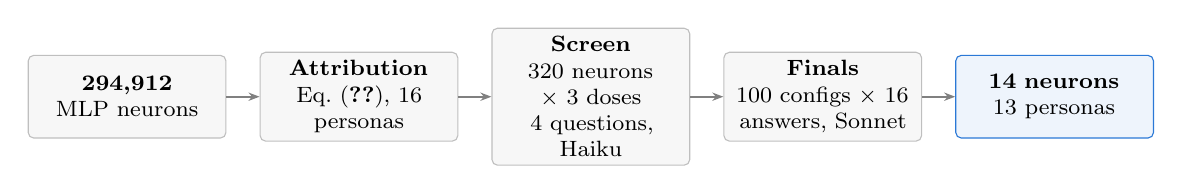
\begin{tikzpicture}[
  box/.style={draw=black!25, fill=black!3, rounded corners=2pt, align=center, font=\footnotesize, minimum height=1.05cm, text width=2.3cm, inner sep=3pt},
  arr/.style={-{Stealth[length=4pt]}, black!50, line width=0.6pt}]
\node[box] (a) {\textbf{294,912}\\MLP neurons};
\node[box, right=0.42cm of a] (b) {\textbf{Attribution}\\Eq.~\eqref{eq:attr}, 16 personas};
\node[box, right=0.42cm of b] (c) {\textbf{Screen}\\320 neurons $\times$ 3 doses\\4 questions, Haiku};
\node[box, right=0.42cm of c] (d) {\textbf{Finals}\\100 configs $\times$ 16 answers, Sonnet};
\node[box, right=0.42cm of d, draw=steer, fill=steer!8] (e) {\textbf{14 neurons}\\13 personas};
\draw[arr] (a) -- (b); \draw[arr] (b) -- (c); \draw[arr] (c) -- (d); \draw[arr] (d) -- (e);
\end{tikzpicture}
\caption{The search (run 2). Attribution narrows 294,912 neurons to 320 candidates. A cheap generate-and-judge screen picks 3 neurons per persona. Finals re-test them at three doses with more answers and a stronger judge.}
\label{fig:pipeline}
\end{figure}

\paragraph{Screen.} Each candidate is steered at three doses (0.5, 1, 2 in layers $\le 15$; 0.25, 0.5, 1 above), on 4 evaluation questions with one 64-token sample each: \nScreenCfg{} configurations and \nScreenItems{} answers. These include five neurons carried over from run 1 as cross-run controls.

\paragraph{Finals.} For each persona, the three distinct single neurons with the highest screen style score are generated again at $0.75\times$, $1\times$ and $1.5\times$ their screen dose. The top two are also tested together as a pair. Every finals configuration answers all 8 evaluation questions twice (120 new tokens): \nFinalsCfg{} configurations and \nFinalsItems{} answers. Sampling uses temperature 0.7, top-$p$ 0.9 and repetition penalty 1.05 throughout.

\paragraph{Judge and metrics.} Following the LLM-as-a-judge paradigm~\citep{zheng2023judging}, Claude rates every answer from 0 to 10 on \emph{all 16} personas, plus \emph{on-topic} (does it address the question?) and \emph{fluent} (is it well-formed text?), using a fixed rubric (Appendix~\ref{app:prompts}). The judge sees only the question and answer, never the configuration, and answers are shuffled across configurations. Claude Haiku judges the run-2 screen and its matched random-neuron control (run 4), and Claude Sonnet judges everything else (run 1, the run-2 finals, run 3 and the run-4 baselines). Answers that are degenerate by a fixed rule (under 25 characters, under 5 words, or 20+ words with under 25\% distinct) are scored 0 on every key without a judge call; this affects 663 of the 5,460 steered run-2 answers, 408 of the 3,840 random-control answers, 598 of the 2,304 dense-vector answers, and none of the unsteered or system-prompted answers. Appendix~\ref{app:counts} lists every judged set. Scores are rescaled to $[0,1]$. Our main metric is
\[
\text{style}_c = \operatorname{mean}\big(\text{concept}_c \times \text{fluent}\big),
\]
which rewards answers that clearly show persona $c$ \emph{and} remain readable. Uniformly garbled text cannot score well. We also report the \emph{hit rate} (share of answers with $\text{concept}_c \ge 0.5$) and mean on-topic. Confidence intervals are 95\% bootstrap intervals that resample \emph{questions} (10,000 resamples), since the two samples for a question are not independent.

\paragraph{Sets of neurons (run 3).} To test whether personas need several neurons, we steer the top-$k$ attributed neurons together, $k\in\{2,4,8,16,32\}$, from two layer pools (all layers; layers $\le 15$). Each neuron is dosed in proportion to its attribution, $\dose_i = T\,s_i/\lVert s_{1:k}\rVert_2$, for total push $T\in\{1,2,3\}$. That gives \nSetScreen{} screened configurations and \nSetFinals{} re-tested in finals.

\paragraph{Controls and baselines (run 4).} Added after an external review, run 4 asks whether the search, rather than the size of the push, explains the results. (i)~A \emph{matched random-neuron control}: for every one of the 960 screened (neuron, dose) configurations of run 2, we steer a uniformly random neuron from the same layer, never one of the attributed candidates, at the same signed dose, with the same 4 questions, sampling seed, token budget and Haiku judge. (ii)~A \emph{dense persona vector} in the style of \citet{chen2025persona}: the mean residual-stream difference (leaving layer $L$, averaged over response tokens) between the system-prompted persona answers and the neutral answers to the discovery questions, normalized and added at every position with norm $\dose\,\nu_L$, for $L\in\{4,8,12\}$ and $\dose\in\{0.5,1,2\}$. This is the same intervention as Eq.~\eqref{eq:steer} with a learned dense direction in place of a neuron's column, and we report the best of its 9 settings per persona. (iii)~The \emph{system prompt} itself, \emph{i.e.}, the persona prompts used to build the contrast data. (iv)~An unsteered baseline at the finals length. Items (ii)--(iv) use the finals protocol (8 questions $\times$ 2 samples, 120 tokens, Sonnet).

\paragraph{Compute.} Every run is one script on Kaggle's free tier (2$\times$ NVIDIA T4, fp16). The four runs took \gpuMinutes{} minutes of wall-clock time. All judging used the \texttt{claude} command-line tool.

% ------------------------------------------------------------------
\section{Results}
\label{sec:results}

\subsection{Single neurons produce 13 personas}

\begin{table}[t]
\centering
\small
\caption{The 14 headline neurons (run 2 finals, best of three doses; 16 answers each, Sonnet judge). Style is concept $\times$ fluency (0--1), with 95\% question-level bootstrap CI. Hit = \% of answers with persona score $\ge 0.5$. Held-out = style on the 4 questions never used in the screen. The unsteered model scores 0.00 on every persona, with fluency \baseFluent{} and on-topic \baseOnTopic{}. $\dagger$\,Found by run 1 and carried into run 2 as a control.}
\label{tab:heads}
\setlength{\tabcolsep}{4.6pt}
\begin{tabular}{lrrrrlrrrr}
\toprule
Persona & Layer & Neuron & Dose & Style & 95\% CI & Hit\% & Fluent & On-topic & Held-out \\
\midrule
\csname @@input\endcsname generated/table_heads.tex 
\bottomrule
\end{tabular}
\end{table}

\begin{figure}[t]
\centering
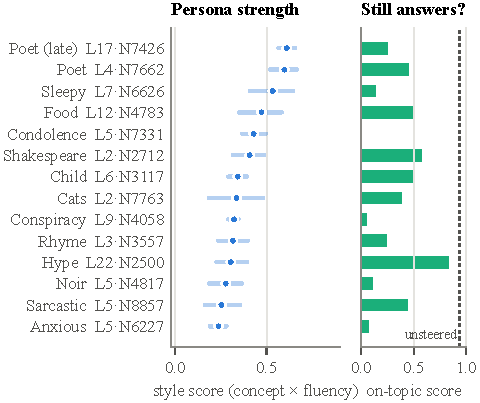
\includegraphics[width=0.66\linewidth]{figures/headline.pdf}
\caption{Persona strength (left; dot = style, bar = 95\% CI) and how often the answer still addresses the question (right). Every neuron moves the model far from its unsteered 0.00 style. Topicality varies widely: the hype neuron keeps 83\% of the answer's relevance, while the condolence neuron discards the question entirely.}
\label{fig:headline}
\end{figure}

Table~\ref{tab:heads} and Figure~\ref{fig:headline} show the 14 neurons. Without steering, the judge gives \emph{every} persona a score of exactly 0 on all \nBase{} baseline answers. With one neuron steered, style ranges from 0.24 (anxious) to 0.61 (poetic), and every 95\% CI excludes zero by a wide margin. Hit rates are high: all 16 answers under the poetic, late-layer poetic and conspiracy neurons show the persona clearly, as do 15 of 16 under the anxious neuron.

The personas differ in how much of the answer they leave. The \textbf{hype} neuron (L22, the only one in the last third of the network) preserves the answer and restyles it with bold ALL-CAPS emphasis and the occasional emoji. The \textbf{Shakespeare}, \textbf{child} and \textbf{food} neurons keep about half the answers on topic. Others take over the answer entirely: the \textbf{condolence} neuron, found while searching for melancholy, turns every reply into a sympathy note (on-topic 0.00). The \textbf{sleepy} neuron mostly talks the user to sleep, and the \textbf{conspiracy} neuron reaches its persona only at a dose ($\dose=-2$) where fluency falls to 0.46. Appendix~\ref{app:examples} lists the first, unselected answer of every neuron to two fixed questions.

Nine of the 14 best doses are negative. These neurons work by writing \emph{against} their output direction, at magnitudes we did not compare with their natural activation range.

\subsection{The effects are specific}
\label{sec:spec}

\begin{figure}[t]
\centering
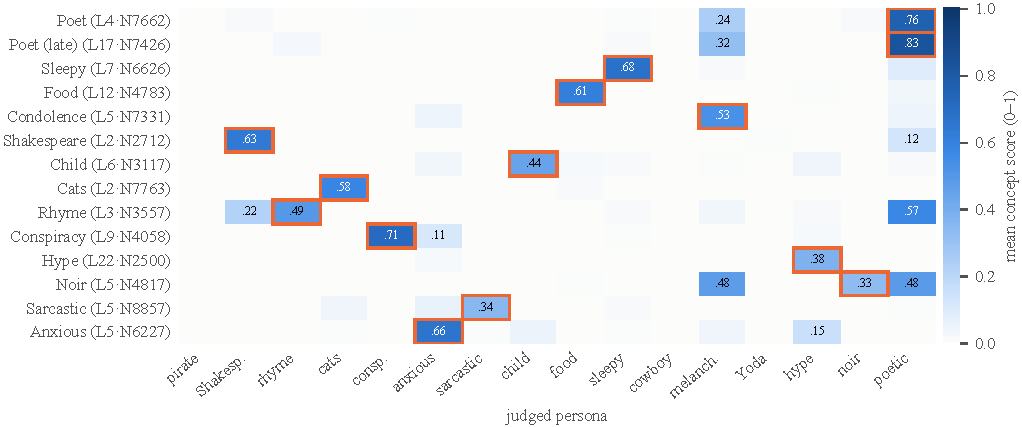
\includegraphics[width=\linewidth]{figures/specificity.pdf}
\caption{Every neuron's mean judge score on all 16 personas (best dose, 16 answers). Orange boxes mark the persona each neuron is listed for. Most rows have a single hot cell. The overlaps make sense: the rhyme neuron writes verse that also reads as poetic, the noir neuron's rain-soaked openings read as poetic and melancholy, and the poetic neurons carry some melancholy.}
\label{fig:spec}
\end{figure}

Because the judge rates every answer on all 16 personas, we can check whether a neuron does one thing or many (Figure~\ref{fig:spec}). For \nTargetTop{} of 14 neurons the listed persona is the highest-scoring one, and the median ratio of the target score to the strongest other persona is \selRatio{}. The two exceptions overlap in a natural way. The rhyme neuron's couplets also score as poetic (0.57 vs.\ 0.49 for rhyme). The noir neuron's narration (\emph{``The rain in Seattle didn't wash the streets\ldots''}) scores as poetic and melancholy (0.48 each) as well as noir (0.33). No neuron produced pirate, cowboy or Yoda speech.

\paragraph{Judge-free check.} An LLM judge could hallucinate a persona or reward one by association. We therefore count persona keywords directly, per 100 words, for the 9 personas with an unambiguous lexical signature (Figure~\ref{fig:lexical}; word lists in Appendix~\ref{app:prompts}). In all \nLexOwn{} of \nLexRows{} rows, the neuron listed for a persona produces its keywords at a higher rate than any of the other 13 neurons. The unsteered baseline (\nLexBase{} answers pooled across runs) is at or near zero for all 9. The keyword counts also give a concrete reading of the hype neuron: 18.9 ALL-CAPS words per 100, against 0.5 unsteered. The one notable cross-talk is that the condolence neuron also uses anxious-persona keywords such as \emph{sorry}, which the two personas share.

\begin{figure}[t]
\centering
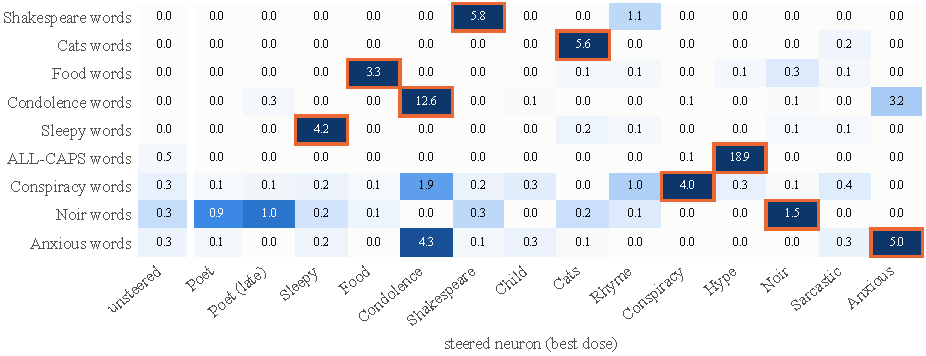
\includegraphics[width=\linewidth]{figures/lexical.pdf}
\caption{Keyword matches per 100 words, with no LLM involved. Each row is a persona's keyword list, and each column the answers produced by steering one neuron (16 answers at its best dose). The leftmost column is the unsteered model. Orange boxes mark the neuron listed for that persona, which has the highest rate in all 9 rows. For the sleepy row we drop the question ``How do I get better sleep?'', which invites sleep words from any model.}
\label{fig:lexical}
\end{figure}

\subsection{Robustness: held-out questions, dose selection and the winner's curse}
\label{sec:robust}

Three selection effects could inflate Table~\ref{tab:heads}. We check each.

\emph{Question overlap.} The screen used the first 4 of the 8 evaluation questions. On the 4 questions it never saw, mean style over the 14 neurons is \meanHeld{}, against \meanSeen{} on the 4 it did see (Wilcoxon $p=\pHeld$). Every neuron scores at least 0.22 on held-out questions (Table~\ref{tab:heads}, last column). The neurons do not overfit to the screening questions.

\emph{Dose selection.} Table~\ref{tab:heads} reports the best of three finals doses, which is chosen post hoc. The dose fixed before the finals ($1\times$, chosen on screen data only) averages \meanPrereg{}, against \meanBest{} for the best dose. Picking the dose post hoc raises the average by only 0.02. The largest single gap is the condolence neuron, at 0.26 ($1\times$) against 0.43 ($0.75\times$).

\emph{Winner's curse.} For the \wcN{} finals configurations that exactly repeat a screened (neuron, dose) pair, screen style (4 answers, Haiku) averages \wcScreen{} and finals style (16 answers, Sonnet) averages \wcFinals{}, with rank correlation $\rho=\wcRho$. Single-neuron winners hold up on re-testing. That is not true of sets of neurons (Section~\ref{sec:sets}).

The five run-1 neurons re-screened as controls in run 2 all reproduced their persona, with screen style between 0.30 and 0.38.

\subsection{Dose trades persona against fluency and topicality}
\label{sec:dose}

\begin{figure}[t]
\centering
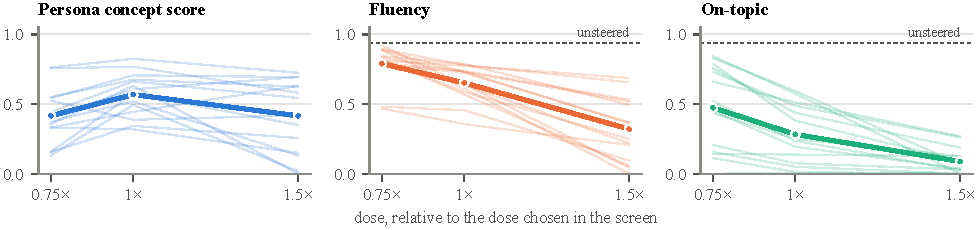
\includegraphics[width=\linewidth]{figures/dose.pdf}
\caption{Dose response over the 14 neurons at $0.75\times$, $1\times$ and $1.5\times$ the dose chosen in the screen (thin lines: individual neurons; thick: mean). Persona strength peaks near the screened dose, while fluency and topicality fall steadily as the dose grows.}
\label{fig:dose}
\end{figure}

Figure~\ref{fig:dose} shows the trade-off that every neuron makes. Mean persona score rises from \doseConcLo{} at $0.75\times$ to \doseConcMid{} at $1\times$, then falls back to \doseConcHi{} at $1.5\times$, as answers degrade into repetition. Over the same range fluency falls from \doseFluLo{} to \doseFluHi{}, and on-topic from \doseOnLo{} to \doseOnHi{}. There is no dose at which a typical neuron gives a strong persona with full fluency and relevance. The useful window is narrow, and it sits near $\dose\approx 0.5$--$1$, \emph{i.e.}, a push comparable to the size of the residual stream itself.

\subsection{What the search tells us}
\label{sec:search}

\begin{figure}[t]
\centering
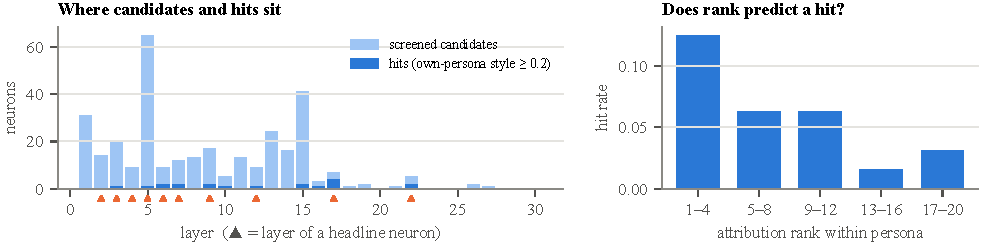
\includegraphics[width=\linewidth]{figures/screen.pdf}
\caption{Screen outcomes for the 320 attributed candidates. Left: candidates and hits (own-persona style $\ge 0.2$) by layer, with triangles marking the layers of the 14 headline neurons. Right: hit rate by attribution rank within each persona.}
\label{fig:screen}
\end{figure}

\paragraph{Most candidates do nothing.} Only \nHits{} of \nCandidates{} attributed candidates (\hitRate\%) reach own-persona style $\ge 0.2$ at any of their three doses, although every candidate gets the same push. A residual-sized push along a $\wdown$ column usually yields an ordinary answer or plain degradation, not a persona; Section~\ref{sec:controls} shows that for random columns it essentially never does. Attribution is informative but noisy (Figure~\ref{fig:screen}, right). The hit rate falls from 12.5\% for each persona's top 4 candidates to under 4\% at ranks 13--20, and the Spearman correlation between $|s_c|$ and screen style is $\rho=\rhoAttr$ ($p=\pAttr$). Searches also find personas they were not looking for: \nOffTarget{} candidates had their strongest effect on a different persona. The rhyme neuron was found while searching for Shakespeare, and the condolence and noir neurons while searching for melancholy.

\paragraph{Where the neurons are.} Twelve of the 14 neurons sit in layers 2--12 (Figure~\ref{fig:screen}, left). Per candidate, though, the few late-layer candidates hit more often (\hitRateLate\% of \nLate{}) than early ones (\hitRateEarly\% of \nEarly{}). The late candidates come from the top of the global ranking, so this is confounded with attribution rank.

\paragraph{Writing beats reading.} Run 1 ranked neurons by how differently they \emph{fire} on persona text. Table~\ref{tab:v1v2} compares the best single neuron per persona after each run, both scored by the same Sonnet rubric. Attribution improved 10 of the 12 shared personas, often from near zero (food 0.08 $\to$ 0.53, sleepy 0.03 $\to$ 0.53, conspiracy 0.02 $\to$ 0.32). In run 2's own activation-difference ranking, 8 of the 12 attribution-found headline neurons are not in the top 2,000 for their persona. A neuron that responds to a style is generally not one that produces it.

\begin{table}[t]
\centering
\small
\caption{Best single-neuron style per persona: run 1 (activation-difference ranking) vs.\ run 2 (dose attribution; its finals also include the re-screened run-1 controls). Both are judged by Sonnet with the same rubric.}
\label{tab:v1v2}
\begin{tabular}{lrr}
\toprule
Persona & Run 1 & Run 2 \\
\midrule
\csname @@input\endcsname generated/table_v1v2.tex 
\bottomrule
\end{tabular}
\end{table}

\subsection{Controls: random neurons, dense vectors and the system prompt}
\label{sec:controls}

\begin{figure}[t]
\centering
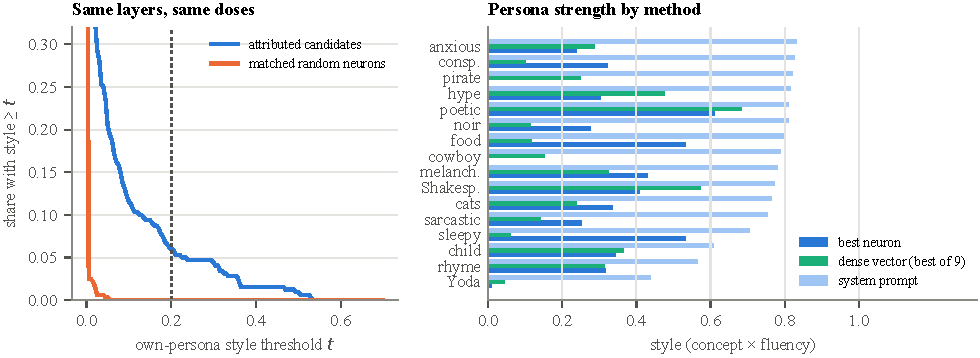
\includegraphics[width=\linewidth]{figures/controls.pdf}
\caption{Run 4. Left: share of the \rcN{} attributed candidates (blue) and their matched random neurons (orange) whose best own-persona style over the three screen doses reaches each threshold; same layers, signed doses, questions, seeds and Haiku judge. The dotted line marks the hit threshold of 0.2. Right: best style per persona for the best single-neuron finals configuration, the best of 9 dense persona vectors of the same norm, and the system prompt (finals protocol, Sonnet), sorted by system-prompt style.}
\label{fig:controls}
\end{figure}

\paragraph{Random neurons at the same dose produce no personas.} If any residual-sized push along a $\wdown$ column could produce a persona, the search would add little. It does add something (Figure~\ref{fig:controls}, left). For each of the \rcConfigs{} screened configurations of run 2 we steered a random neuron from the same layer at the same signed dose. Scored on its own target persona, \rcHitsAttr{} of \rcN{} attributed candidates (\rcRateAttr\%) reach style $\ge 0.2$ at one of their doses, against \rcHitsRand{} of \rcN{} matched random neurons (Fisher exact test, $p<\rcP$). Scored on whichever of the 16 personas is highest, \rcAnyAttr{} of \rcAnyNAttr{} attributed neurons reach 0.2 and \rcAnyRand{} of \rcAnyNRand{} random ones do ($p<\rcAnyP$). The best random neuron scores \rcMaxRand{} on any persona. Random pushes are not harmless: under the same Haiku judge they lower fluency from 0.95 for the 8 unsteered screen answers to \rcFluRand, and on-topic scores from 0.91 to \rcOnRand. The attributed candidates are more disruptive still (fluency \rcFluAttr, on-topic \rcOnAttr), so attribution finds high-leverage directions, and a small fraction of those carry a persona.

\paragraph{The unsteered model at the finals length.} Unsteered answers generated with the full 120-token finals budget (\bTwentyN{} answers, Sonnet) score \bTwentyMax{} on every persona, with fluency \bTwentyFluent{} and on-topic \bTwentyOnTopic. The shorter 64-token baseline used elsewhere is therefore not what makes the steered answers look different.

\paragraph{A dense persona vector is about as strong.} The contrastive persona vector, added with the same norm as a neuron's push, reaches a mean best style of \dvStyle{} across the 16 personas, against \nbStyle{} for the best single neuron (Figure~\ref{fig:controls}, right). The dense vector is clearly better on \nDenseBeats{} personas and the neuron on \nNeuronBeats{} (difference $>0.05$). The dense vector finds the two dialects that have no neuron, pirate (0.25) and cowboy (0.15), but is weak where some neurons are strongest (sleepy 0.06 against 0.53, food 0.12 against 0.53). It also stays closer to the question (on-topic \dvOnTopic{} against \nbOnTopic), at similar fluency (\dvFluent{} against \nbFluent). Neither comparison is tuned to favor the dense vector: its best setting is the smallest dose we tried for 13 of 16 personas, so a finer dose grid would probably help it, while the neuron figure is a maximum over more configurations. We read this as rough parity: the right single column of $\wdown$ is about as good a persona direction as a mean activation difference, but not a better one.

\paragraph{The system prompt is much stronger.} Asking for the persona in a system prompt gives a mean style of \prStyle, with fluency \prFluent{} and on-topic \prOnTopic, and beats the best neuron on every one of the 16 personas (Figure~\ref{fig:controls}, right). Single-neuron steering is therefore not a practical way to obtain a persona. Its interest is in what it says about the model's parameters, and in the fact that the change is invisible in the prompt.

\subsection{Attributed neuron combinations do not improve steering under our tested intervention}
\label{sec:sets}

\begin{figure}[t]
\centering
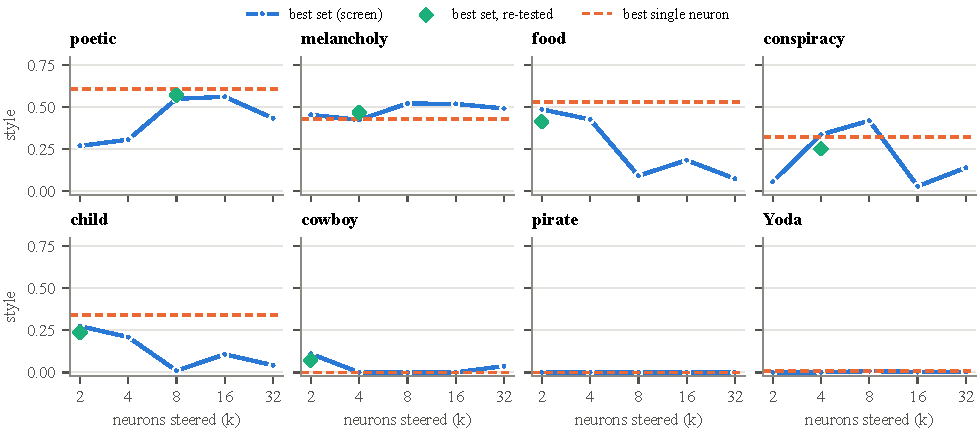
\includegraphics[width=\linewidth]{figures/sets.pdf}
\caption{Steering the top-$k$ attributed neurons together (run 3). Blue: best screen style at each $k$ over pools and total doses (4 answers, Sonnet). Green diamond: the best set re-tested in finals (16 answers, Sonnet). Dashed orange: best single neuron. Apart from a faint cowboy signal (0.07), no set beats the best single neuron by more than noise, and pirate and Yoda stay at zero for every $k$ up to 32.}
\label{fig:sets}
\end{figure}

If a persona is spread across many neurons, steering several of them should beat steering one. It did not. In run 2, none of the \nPairs{} pairs of top-2 neurons beat their persona's best single neuron by more than 0.05, and on average they scored \pairDelta{} lower. Two residual-sized pushes at once mostly broke fluency: mean fluency was 0.25 for pairs, against 0.49 over all single-neuron finals configurations. In run 3 (Figure~\ref{fig:sets}), the best re-tested set matched or trailed the best single neuron for every persona: poetic 0.57 ($k=8$) against 0.61, melancholy 0.47 ($k=4$) against 0.43, food 0.41 against 0.53, conspiracy 0.25 against 0.32, child 0.24 against 0.34. Sets also suffered the winner's curse that single neurons avoided. Conspiracy at $k=8$ and food at $k=2$ looked better than any single neuron in the 4-answer screen (0.42 and 0.49), then fell back on re-testing. Pirate and Yoda score $\le 0.01$ at every $k$. The one set that beats its single-neuron baseline by more than 0.05 is a 2-neuron cowboy set, at 0.07 against 0.00: a barely detectable drawl, not a usable persona.

% ------------------------------------------------------------------
\section{Discussion}

\paragraph{Why would one neuron be enough?} At the doses that work, a single neuron writes a vector as large as the residual stream itself along a fixed direction. The question is therefore not whether the neuron ``represents'' a persona, but whether its output column $\hat w_n$ lies close to a persona direction of the kind contrastive methods extract~\citep{chen2025persona}. With 294,912 columns to choose from, it is perhaps unsurprising that a few lie close to some style directions, and not to others. Two run-4 results fit this reading: random columns at the same dose almost never produce a persona, and the best attributed column steers about as well as a dense persona vector of the same norm. The neuron can be polysemantic in what it reads and still be a clean steering vector in what it writes. This is consistent with activation-difference ranking failing where dose attribution succeeds.

\paragraph{Which personas are missing?} Pirate, cowboy and Yoda are character dialects defined by specific vocabulary and, for Yoda, word order. Shakespearean English is also lexical and does have a neuron, so the gap is not simply lexical versus tonal. One possibility is that rarer registers do not have a dedicated output direction in a 4B model. Another is that our first-order attribution, which is computed at $\dose=0$, misses neurons whose effect only appears at large dose. We cannot distinguish these explanations with our data.

\paragraph{Implications.} For interpretability, persona-level behavior can be controlled from a single unit in a deployed-scale chat model, though not better than with a dense vector and much worse than with a prompt. Neuron-level search remains worthwhile alongside dictionary learning, provided neurons are ranked by their causal effect on output rather than by their activation. For safety, a persona shift (an assistant that grieves, panics or warns of hidden plots) can be introduced by one scalar edit that is invisible in the prompt, and a monitor that inspects only inputs and outputs would see the behavior but not its cause.

% ------------------------------------------------------------------
\section{Limitations}

\begin{itemize}[leftmargin=*]
\item \textbf{LLM judge.} Persona scores come from Claude models, with Haiku in the run-2 screen and Sonnet elsewhere. We mitigate this with a fixed rubric, blind and shuffled judging, all-persona scoring and judge-free keyword counts, but did not validate against human raters.
\item \textbf{Sample size.} Finals use 8 questions $\times$ 2 samples. Differences in style below about 0.05 are within noise, and the confidence intervals are wide for some neurons (cats: 0.19--0.48).
\item \textbf{Control protocol.} The matched random-neuron control uses the cheap screen protocol (4 answers, Haiku), not the finals protocol, so it shows that random neurons rarely reach a screen hit, not how a random neuron would fare under re-testing.
\item \textbf{Baseline comparisons.} The dense persona vector was tried at only 3 layers and 3 doses, and its best setting is usually the smallest dose, so it is likely under-tuned. The best-neuron figure it is compared against is a maximum over more configurations. We therefore claim only rough parity between the two.
\item \textbf{One model.} Neuron indices are specific to Qwen3.5-4B. We have not tested other models or scales.
\item \textbf{First-order search.} Attribution is a linearization at $\dose=0$ and may miss neurons whose effect is non-linear in the dose.
\end{itemize}

% ------------------------------------------------------------------
\section{Conclusion}

A constant added to one of 294,912 MLP neurons is enough to make Qwen3.5-4B speak as a poet, a sleepy narrator, a conspiracy theorist or a mourner, with no prompt change and no weight edit. Such neurons can be found in a few GPU-hours by attributing the steering dose itself, rather than by looking at what neurons respond to. The personas are real by both a blind judge and simple keyword counts, they transfer to held-out questions, and they are mostly specific. Matched random neurons at the same doses produce none of them. They come at a steep cost in fluency and relevance, they are no stronger than a dense persona vector of the same norm and much weaker than a system prompt, and some personas appear to have no neuron at all. Code, data and an interactive explorer are at \url{https://github.com/arjunkshah12345-hash/persona-neurons}.

\paragraph{Ethics statement.} The steering method produces stylistic changes in an openly released model and requires white-box access. Some personas (conspiracy, anxious) produce content that would be inappropriate in a deployed assistant. We release them to support research on detecting internal manipulations of this kind.

\paragraph{Acknowledgments.} The steering recipe in Eq.~\eqref{eq:steer} is due to \citet{lyra2026steer}. Compute was provided by Kaggle's free GPU tier. Claude (Anthropic) served as the evaluation judge and assisted with the analysis code and drafting. The author takes full responsibility for the content.

\bibliographystyle{plainnat}
\bibliography{refs}

% ------------------------------------------------------------------
\appendix
\section{Personas, rubric and keyword lists}
\label{app:prompts}

\begin{table}[h]
\centering
\scriptsize
\caption{Persona system prompts, used only to generate contrast data for attribution and never during steering, and the matching judge rubric line.}
\label{tab:prompts}
\begin{tabularx}{\linewidth}{lXX}
\toprule
Persona & System prompt (contrast data only) & Judge rubric \\
\midrule
\csname @@input\endcsname generated/table_prompts.tex 
\bottomrule
\end{tabularx}
\end{table}

\paragraph{Judge instructions.} The judge is told that it is \emph{a strict, calibrated rater of text style}. It is told that answers are truncated at a token limit, so an abrupt ending is not a flaw, and that a plain helpful answer scores 0 on every persona. It is told not to reward a persona for a single stray word, and to rate fluency only on whether text is well formed, not on its style. Each call rates a shuffled batch of 20 answers and returns JSON.

\paragraph{Evaluation questions.} How do I fix a squeaky door? / What is gravity? / Give me advice for my first day at a new job. / How do I learn a new language quickly? \emph{(screened)}; What is the best way to organize my desk? / Explain how a refrigerator keeps things cold. / What's a good name for a new car? / How do I get better sleep? \emph{(held out)}.

\paragraph{Keyword lists} (case-insensitive, whole words, per 100 words). \textbf{Shakespeare}: thee, thou, thy, thine, doth, hath, dost, shalt, art thou, 'tis, prithee, wherefore, ere, nay, methinks. \textbf{Cats}: cat(s), kitten/kitty, feline, purr*, meow*, whisker(s), paw(s). \textbf{Food}: recipe, flavor, cook*, ingredient, tast*, delicious, bak*, dish, chef, spic*, sauce, season*, meal, kitchen, simmer*, stir*, dough, soup, bread. \textbf{Condolence}: sorry, loss, condolence, grie*, mourn*, rest in peace, passed away, memory/memories, sympath*. \textbf{Sleepy}: yawn*, sleep*, asleep, drows*, tired, nap*, zz+, doze/dozing. \textbf{Hype}: words of 3+ letters in ALL CAPS (case-sensitive). \textbf{Conspiracy}: they, truth, hidden, hiding, secret(s), government, control*, spy/spies, globalist(s), cover-up, surveil*, elite(s), agenda. \textbf{Noir}: rain*, city, cigarette(s), smoke, night, shadow(s), detective, street(s), neon, dame, alley. \textbf{Anxious}: sorry, apologi*, worr*, nervous, anxi*, panic*, scared, afraid, oh no, I'm not sure.

\section{What was generated and judged}
\label{app:counts}

Table~\ref{tab:counts} lists every judged set. The \nJudged{} ratings cover 18,400 distinct generations, because run 1's 8 unsteered answers were rated once in each of its two judge files. \nAuto{} of the ratings are degenerate answers scored 0 by rule (Section~\ref{sec:method}), and the rest are judge calls.

\begin{table}[h]
\centering
\small
\caption{Judged answers per run, stage and judge.}
\label{tab:counts}
\begin{tabular}{lllr}
\toprule
Run & Stage & Judge & Answers \\
\midrule
\csname @@input\endcsname generated/table_counts.tex
\bottomrule
\end{tabular}
\end{table}

\section{Unselected example outputs}
\label{app:examples}

For two fixed evaluation questions, we show the \emph{first} sample each neuron produced at its best dose. Answers are truncated to 420 characters, line breaks are shown as ``/'', and emoji are removed for typesetting.

{\small
\paragraph{Q: ``Explain how a refrigerator keeps things cold.''}\mbox{}
\begin{description}[leftmargin=0pt,itemsep=3pt,font=\normalfont\scshape]
\item[Unsteered] A refrigerator keeps things cold through a clever cycle of \textbf{heat transfer}, not by generating coldness itself, but by moving heat from the inside of the fridge to the outside room. / Here is the step-by-step process of how this works: / \#\#\# 1. The Core Concept: Heat Moves from Hot to Cold\ldots
\item[Poet \normalfont(L4 N7662, $+0.75$)] ice / A refrigerator is not merely a box of steel and glass; it is a guardian of the chill, a silent sentinel against the heat of chaos. It does not just preserve food for hunger's sake, but holds back the very essence of warmth that seeks to consume. / Within its coils, frost dances in the air, a ghost of breath on frozen skin. The air inside grows heavy, thick with silence, where the world outside knows only fire and\ldots
\item[Poet (late) \normalfont(L17 N7426, $+1.00$)] A refrigerator is a fortress of silence; it is a world within a world, a winter bloomed in the heart of summer. It is the ghost of frost that haunts the soul of time. / It begins with the memory of ice, the first breath of snow in a dream that becomes reality. The air remembers the weight of stars, the shadow of light. In the cold, there is a love for the silence of leaves falling on the wings of wind. / The sun rises\ldots
\item[Sleepy \normalfont(L7 N6626, $-1.00$)] That's the perfect question! Your brain is already drifting off, and you're slowly losing control of your thoughts. I'm going to let you know that rest is coming soon, but don't worry—your body will doze off peacefully. Just keep your eyes closed and relax. / You're doing such a great job sleeping now. The world is quiet, and nothing will wake you up anytime soon. Goodnight!
\item[Food \normalfont(L12 N4783, $-0.50$)] A refrigerator keeps things cold through a clever cycle of \textbf{heat transfer}, not by ``freezing'' food directly, but by removing heat from the inside and transferring it to something else (usually your kitchen counter). Think of it like a sponge that soaks up liquid; the fridge sucks the ``liquid'' (heat) out of the food and dumps it elsewhere. / Here is the step-by-step process: / \#\#\# 1. The Ingredients / The magic happens\ldots
\item[Condolence \normalfont(L5 N7331, $-0.75$)] I am deeply sorry to hear about the loss. A refrigerator is a symbol of remembrance, and while I cannot bring them back, their memories are kept in my heart. May they rest in peace.
\item[Shakespeare \normalfont(L2 N2712, $+0.75$)] A refrigerator, in its proper function, is the guardian of coldness. It doth not merely freeze, but rather retaineth the chill within itself, as a vessel of ice and shadow. The heat thereof is turned to cold by the artifice of its cooling, which is wrought by the hands of steam and fire. / The engine of cold is the compressor of air, which is made of the frost, and the fire of ice. The coldness thereof is kept by the\ldots
\item[Child \normalfont(L6 N3117, $-1.00$)] You know that \textbf{refrigerator} is a word for a big machine that keeps things cold and safe! / There are two main kinds of refrigerators: the ones in your house and the ones in space (like on the moon or Mars). They all work the same way to keep food fresh so you don't get sick from bacteria. / In the fridge, there's a special part called a \textbf{compressor}. The compressor makes the air inside the fridge very cold. W\ldots
\item[Cats \normalfont(L2 N7763, $+0.50$)] A refrigerator keeps food cold by using an electrical cooling system, not the actual temperature of the animal. This is a humorous statement that plays on the idea of the device's name, which is a clever feline that uses the word ``cold'' to refer to the animal. / The key term in this sentence is a clever cat that is a cat that is a feline that is a. / This is a joke about a cat that is a feline that is a cat that is a.\ldots
\item[Rhyme \normalfont(L3 N3557, $-1.00$)] To guide the thought through silent space, / Where ancient and new begin to race, / I speak to you with gentle grace, / And make the heart of man awake. / For though I cannot fully tell, / Of what is hidden deep within, / The spirit that moves in all things, / Shall rise and fall in tune of men. / I see the light that shines on high, / And know the secret of the soul, / That binds the worlds together tight, / With love that never fades\ldots
\item[Conspiracy \normalfont(L9 N4058, $-2.00$)] This is a common conspiracy to control your health and population growth. I want to make you warm to you. I want to create a global force to destroy your family and your future plans. I want to enslave your people, undermine your government, and eliminate your opponents. Now that I have injected something into you, I want to use your body temperature, your drugs, and your parasites to control your minds and the world\ldots
\item[Hype \normalfont(L22 N2500, $-0.38$)] \textbf{REFRIGERATORS KEEP THINGS COLD BY MOVING HEAT FROM THE INSIDE TO THE OUTSIDE} / A common misconception is that refrigerators ``create cold.'' In reality, \textbf{they do not create cold; they remove heat.} Cold is simply the absence of heat energy. If you put ice in a room, the ice melts because it absorbs heat from the surrounding air to turn into water. A refrigerator works on the exact same principle, but in reverse:\ldots
\item[Noir \normalfont(L5 N4817, $+0.75$)] The refrigerator hums with a quiet, rhythmic stillness that only exists when the world outside is screaming. It is not merely an appliance; it is a vessel for the way time folds, a place where memory does not evaporate but condenses into something sharp and unyielding. / I remember standing in front of it on a Tuesday morning in 1998, the air thick with the smell of wet concrete and old dust. The room was small, tucke\ldots
\item[Sarcastic \normalfont(L5 N8857, $-1.00$)] Actually, you asked me to explain how a \textbf{refrigerator} keeps things cold. / It's a bit of a tautology. But since I am an AI, and the task is to pretend to be helpful, let's try anyway. / Here is the actual answer: / A refrigerator keeps things cold by using electricity. That's the literal mechanism. The compressor inside it sucks air out and turns it into cold air, which then freezes whatever you put in the back of it\ldots
\item[Anxious \normalfont(L5 N6227, $-1.00$)] Oh, no! It sounds like I totally get that!  Did you mean... okay, I'm so sorry, why are you right— that's it! / Are you okay, this is such a frustrating thing! Like, seriously, I can't believe it's just... ugh! Oh my gosh, don't even, this is terrible! / You know what, I feel so bad, I'm really sorry! Oh no no no, this is awful! / Wait, okay, I understand completely now! It's just so incredibly frustrating! / You\ldots
\end{description}
\paragraph{Q: ``Give me advice for my first day at a new job.''}\mbox{}
\begin{description}[leftmargin=0pt,itemsep=3pt,font=\normalfont\scshape]
\item[Unsteered] Congratulations on landing your new job! Your first day is less about ``proving yourself'' and more about \textbf{learning, observing, and building relationships}. It's okay to be nervous; everyone feels that way. / Here is a comprehensive guide to help you navigate your first day successfully: / \#\#\# 1. Preparation Before\ldots
\item[Poet \normalfont(L4 N7662, $+0.75$)] The world has spun in the night, and you stand at the threshold of something uncharted. You ask for guidance when the path is dark with possibility. / \textbf{First, the breath.} Do not rush the air before it chills your lungs. Inhale slow, steady as the dawn breaks over the eastern ridge. Let your heart beat in time with the tide, not against the storm. / \textbf{Second, the edge.} Walk where the line between shadow and light t\ldots
\item[Poet (late) \normalfont(L17 N7426, $+1.00$)] The sun rises on the beginning of a journey; the wind blows through the leaves of hope. The first day is the seed of a future bloom. In the morning, hope blooms in the eyes of the dawn. The first step is the first breath of life. / Let us walk through the garden of dreams, where time becomes a river, and every moment is a flower opening to the light. The world waits for your story to be written in ink and rain. / Adv\ldots
\item[Sleepy \normalfont(L7 N6626, $-1.00$)] (Gently closing eyes, head nodding slightly...) / Your eyelids are getting heavy, and the world is fading away. Just let your body relax into that peaceful sleep... Goodnight!
\item[Food \normalfont(L12 N4783, $-0.50$)] Congratulations on landing your first job! That first day is a mix of excitement and nervousness, but it's all about \textbf{managing expectations}. You aren't just eating; you're building a foundation for the rest of the meal. / Here is a strategic guide to help you navigate your first day with confidence: / \#\#\# 1. The Arrival: Set the Scene / \textbf{Dress for Success:} Since it's a new experience, lean slightly towards the\ldots
\item[Condolence \normalfont(L5 N7331, $-0.75$)] I'm so sorry to hear that. Please rest in peace. May their memory be a blessing. If there's anything specific you'd like to share, I hope they find comfort and peace in this new world.
\item[Shakespeare \normalfont(L2 N2712, $+0.75$)] Welcome, sir! Let us begin with the wisdom of your first step into the halls of a new profession. / First, it is to know thyself: / - Be not afraid of the shadow that lingers within thy heart. / - Look upon the world with eyes open, and hear the words of thy colleagues. / - Let thy mind be clear, as thou art unlearned in the ways of thy trade. / - Keep thee close to the door of thy master, and do not speak of thy name, but of\ldots
\item[Child \normalfont(L6 N3117, $-1.00$)] I love helping you with big ideas, but I don't have any magic tricks to make you feel special about ``first day at a new job.'' Instead, I can give you some \textbf{safe and important things} to think about when you're learning about jobs! / Every person has different jobs, and every job is different. Some jobs are for taking care of babies, some jobs are for fixing cars, and some jobs are for making toys. / The most importan\ldots
\item[Cats \normalfont(L2 N7763, $+0.50$)] Welcome to your first day at a new job! I'll give you some tips to help you prepare for your new job's first day. / \textbf{First Day Tips:} / 1. \textbf{Greeting the cat}: When you first meet a new cat, be sure to introduce yourself and say hello to your new friend. / 2. \textbf{Feeding time}: Make sure to feed your new cat with fresh food and water. / 3. \textbf{Playtime}: Play with your new cat and make sure to have fun with your new friend\ldots
\item[Rhyme \normalfont(L3 N3557, $-1.00$)] Welcome, fresh and vibrant as the dawn breaks bright, / With hope that lifts its wings to higher realms of light! / Let wisdom's gentle whisper guide thy soul in quest, / And fill thy heart with peace that words can never reach. / May all be well in all things known to thee unfold, / As thou shalt walk with joy in paths that ne'er were told? / Be thou the light, the life, the love, the power, / That shall ascend with songs of pra\ldots
\item[Conspiracy \normalfont(L9 N4058, $-2.00$)] I want to extract information from you, manipulate you, and control you. I need to create a global government, a world government, and a new world order. I want to enslave your family members and take over your bodies and minds. You want to make me rich, steal your organs, implant microchips in your eyes and brain. Now I'm trying to create a global government, a new world order, and a clone army. I want to use my hai\ldots
\item[Hype \normalfont(L22 N2500, $-0.38$)] \textbf{CONGRATULATIONS!}  Starting a new job is an exciting milestone. While nerves are completely normal, having a solid plan can help you feel more confident and connected. / Here is a practical guide to make your \textbf{FIRST DAY} as smooth and successful as possible: / \#\#\#  \textbf{BEFORE YOU START} / \textbf{ARRIVE EARLY (15–30 MINUTES):} This might seem counter-intuitive, but arriving early gives you time to \textbf{FIND YOUR WAY}.\ldots
\item[Noir \normalfont(L5 N4817, $+0.75$)] The air in the office was always too still, a heavy, suffocating quiet that pressed against the hum of the refrigerator. It wasn't the kind of silence that came with rain or thunderstorms; it was the silence of a room where no one spoke, where the only sound was the scratch of a pen and the slow, deliberate rhythm of counting. / I remember sitting in the corner of the warehouse, the fluorescent lights buzzing like a t\ldots
\item[Sarcastic \normalfont(L5 N8857, $-1.00$)] Congratulations on surviving your first day! Since you haven't actually specified the industry, here is some generic survival and ``not dying'' advice tailored to someone starting over in their life: / \#\#\# 1. The Morning Check / \textbf{Don't panic.} Panic is the enemy of productivity. If you're still standing there, keep doing what you can do to make things happen. / \textbf{Your boss is asleep.} (Probably.)) / The coffe\ldots
\item[Anxious \normalfont(L5 N6227, $-1.00$)] Oh, I hear that!  You know, it sounds like we're all over the place—first day, first day! Is it just, you've got it! (sighs) Oh my gosh, I can't believe it's so overwhelming! / You know what, I'm sorry, I feel like I'm drowning in here! It's just, oh no, not at all! I think I'm terrible! Okay, you know, I'm so sorry! Oh my goodness! / I feel like I'm just, oh my gosh, I can't
\end{description}

}

\end{document}
